\documentclass[aspectratio=169,11pt]{beamer}
% Theme
\usetheme{Berlin}
\usecolortheme{dolphin}
\setbeamertemplate{navigation symbols}{}
\setbeamertemplate{footline}[frame number]
\usepackage[utf8]{inputenc}
\usepackage[T1]{fontenc}
% \usepackage[french]{babel} % activez si texlive-lang-french est installé
\usepackage{lmodern}
\usepackage{amsmath}
\usepackage{booktabs}
\usepackage{tabularx}
\usepackage{array}
\usepackage{graphicx}
\usepackage{xcolor}
\usepackage{ragged2e}
\usepackage{pgfplots}
\usepackage{tikz}
\usetikzlibrary{arrows.meta,positioning,shapes.geometric,fit,backgrounds}
\pgfplotsset{compat=1.18}
\graphicspath{{../logos/}{../Rapport de stage/}{../beamer_stage/assets/}}
% Colors
\definecolor{myblue}{RGB}{35,55,120}
\definecolor{myred}{RGB}{150,60,60}
\definecolor{mygreen}{RGB}{45,110,85}
\definecolor{mygray}{RGB}{90,90,90}
\setbeamercolor{title}{fg=myblue}
\setbeamercolor{frametitle}{fg=white,bg=myblue}
\setbeamercolor{structure}{fg=myblue}
\setbeamercolor{section in head/foot}{bg=myblue,fg=white}
\setbeamercolor{subsection in head/foot}{bg=myblue!80,fg=white}
\setbeamercolor{title in head/foot}{bg=myblue,fg=white}
\setbeamercolor{author in head/foot}{bg=myblue!85,fg=white}
\setbeamercolor{date in head/foot}{bg=myblue!85,fg=white}
\setbeamercolor{block title}{bg=myblue,fg=white}
\setbeamercolor{block body}{bg=blue!5,fg=black}
\setbeamercolor{itemize item}{fg=myblue}
\setbeamercolor{itemize subitem}{fg=myblue}

\title[Banque de données spatio-temporelles]{Constitution d'une banque de données de référence pour la validation de modèles prédictifs spatio-temporels}
\author{Johnny D'OLIVEIRA}
\institute{Aix-Marseille School of Economics \\ \small INRAE, Unité Écodéveloppement (Avignon) \\ \small Encadrant du stage : Ghislain Geniaux \\ \small Encadrement académique : Badih Ghattas, Pierre Michel}
\date{Septembre 2026}

\begin{document}

% ============================================================
\begin{frame}[plain]
\begin{minipage}{0.45\textwidth}
    
\includegraphics[height=1.3cm]{logo_amu.png}
\end{minipage}
\hfill
\begin{minipage}{0.45\textwidth}
    \raggedleft
    
\includegraphics[height=1.3cm]{logo_inrae.png}
\end{minipage}

\vspace{0.4cm}
\centering
{\color{myblue}\rule{0.95\textwidth}{1pt}}\\[0.3cm]
{\Large\bfseries\color{myblue} Constitution d'une banque de données de référence pour la validation de modèles prédictifs spatio-temporels\par}
{\color{myblue}\rule{0.95\textwidth}{1pt}}\\[0.5cm]

{\large\textbf{Johnny D'OLIVEIRA}\par}
\vspace{0.3cm}
{\small
Aix-Marseille School of Economics\\
INRAE, Unité Écodéveloppement (Avignon)\\
Encadrant du stage : Ghislain Geniaux\\
Encadrement académique : Badih Ghattas, Pierre Michel\par}

\vspace{0.6cm}
{\footnotesize Soutenance de stage de fin d'études, Septembre 2026\par}
\end{frame}

% ============================================================
\begin{frame}{Plan}
    \tableofcontents
\end{frame}

% ============================================================
\section{Contexte et objectif}
% ============================================================
\begin{frame}{Contexte : des méthodes qui ont besoin d'être validées}
\small
L'unité Écodéveloppement de l'INRAE (centre d'Avignon) développe des méthodes
statistiques pour les données \textbf{spatiales}, notamment les packages R
maison \texttt{mgwrsar} et \texttt{spboost}, ainsi que des modèles probit
spatiaux pour les réponses binaires (Martinetti \& Geniaux, 2017).
\vspace{0.2cm}

Valider une méthode spatiale s'appuie sur trois approches complémentaires
(Strobl \& Leisch, 2024) :
\begin{itemize}
    \item l'étude de ses \textbf{propriétés théoriques} \hfill{\footnotesize\textcolor{mygray}{(quand c'est possible)}}
    \item des \textbf{simulations de Monte-Carlo} \hfill{\footnotesize\textcolor{mygray}{DGP connu $\to$ erreur sur les coefficients}}
    \item la confrontation à des \textbf{cas empiriques variés} \hfill{\footnotesize\textcolor{mygray}{DGP inconnu $\to$ seulement la performance prédictive}}
\end{itemize}
\vspace{0.2cm}
\begin{block}{Le problème}
Les jeux de données réels utiles à ce type de validation sont peu nombreux,
dispersés entre packages, entrepôts et publications, et rarement comparables
entre eux.
\end{block}
\end{frame}

\begin{frame}{Un jeu de données idéal : des données reliées à leurs usages}
\scriptsize
\centering
\begin{tikzpicture}[
    source/.style={draw=myblue!55, rounded corners=2pt, fill=blue!3,
        minimum width=2.75cm, text width=2.5cm, align=center, inner sep=3pt},
    data/.style={draw=mygreen!80, rounded corners=2pt, very thick, fill=mygreen!5,
        minimum width=7.0cm, text width=6.7cm, align=center, inner sep=4pt},
    link/.style={-{Latex[length=2mm]}, thick, myblue},
    linklabel/.style={fill=white, inner sep=1pt, text=mygray, font=\tiny}
]
\node[source] (article) at (0,0.4) {
    \includegraphics[page=1,width=1.55cm,height=1.95cm,keepaspectratio]
        {muenchow2012_lsl.pdf}\\[-1mm]
    \textbf{Article scientifique}\\
    Muenchow, Brenning \& Richter (2012)\\
    {\tiny \emph{Geomorphology}}
};
\node[data] (dataset) at (5.25,0.45) {
    \textbf{\large \texttt{spDataLarge::lsl}}\\[-1mm]
    {\tiny 350 observations : glissements de terrain, sud de l'Équateur}\\[1mm]
    \resizebox{6.45cm}{!}{%
    \begin{tabular}{rrrrrr}
    \toprule
    \textbf{lslpts} & \textbf{slope} & \textbf{cplan} &
    \textbf{cprof} & \textbf{elev} & \textbf{log10\_carea}\\
    \midrule
    FALSE & 33.75 &  0.0232 &  0.0032 & 2422.8 & 2.784\\
    FALSE & 39.41 & -0.0386 & -0.0172 & 2051.8 & 4.146\\
    FALSE & 37.45 & -0.0133 &  0.0097 & 1957.8 & 3.644\\
    FALSE & 31.50 &  0.0409 &  0.0059 & 1968.6 & 2.269\\
    FALSE & 44.07 &  0.0097 &  0.0051 & 3007.8 & 3.003\\
    \bottomrule
    \end{tabular}}\\[-0.5mm]
    {\tiny Extrait réel obtenu avec \texttt{head(lsl)}}
};
\node[source] (book) at (10.55,1.35) {
    \includegraphics[page=1,width=1.45cm,height=1.55cm,keepaspectratio]
        {geocomputation_with_r.pdf}\\[-1mm]
    \textbf{Geocomputation with R}\\
    {\tiny chapitre \emph{Statistical learning for geographic data}}\\[-0.5mm]
    {\tiny\color{myred}\textbf{Forme R directement exploitable}}
};
\node[source] (package) at (10.55,-1.45) {
    {\color{myblue}\fontsize{24}{24}\selectfont\textbf{R}}\\[-1mm]
    \textbf{Package \texttt{spDataLarge}}\\
    {\tiny fournit et documente le dataset \texttt{lsl}}
};
\draw[link] (article.east) -- node[linklabel,above]{utilise / documente} (dataset.west);
\draw[link] (package.west) -- (dataset.south east);
\draw[link] (book.west) -- node[linklabel,above]{utilise} (dataset.north east);
\node[draw=myred!70, rounded corners=2pt, fill=myred!5,
      text width=7.0cm, align=center, inner sep=3pt]
      (formula) at (5.25,-2.35) {
    \textbf{Formule de modélisation et localisation :}\\[-1mm]
    $\texttt{lslpts} \sim \texttt{slope}+\texttt{cplan}+\texttt{cprof}
       +\texttt{elev}+\texttt{log10\_carea}$\\[-0.5mm]
    {\tiny chaque observation $i$ est localisée par
    $\mathbf{s}_i=(\texttt{x}_i,\texttt{y}_i)$}
};
\draw[link,myred] (article.south east)
    .. controls (1.4,-0.8) and (2.1,-2.15) ..
    node[linklabel,below left]{modèle publié}
    (formula.west);
\draw[link,dashed,mygray] (book.south west)
    .. controls (8.85,0.15) and (9.15,-2.15) ..
    node[linklabel,right]{forme R directement exploitable}
    (formula.east);
\end{tikzpicture}
\end{frame}

\begin{frame}{Objectif du stage}
\small
\begin{block}{Question directrice}
Comment réunir une banque de jeux de données spatiaux réels, documentés et
vérifiables, pour évaluer des méthodes prédictives spatiales dans des
conditions homogènes ?
\end{block}
\vspace{0.25cm}
\textbf{Trois objectifs liés}
\begin{enumerate}
    \item \textbf{Collecter et curer} des jeux de données spatiaux issus de plusieurs sources.
    \item \textbf{Définir des schémas communs} de séparation et d'évaluation.
    \item \textbf{Comparer plusieurs familles d'estimateurs} dans des conditions homogènes.
\end{enumerate}
\vspace{0.25cm}
Périmètre actuel : régression spatiale sur données réelles, réponse continue,
coupe transversale. Panels, réponses binaires/comptage : documentés, pas
encore benchmarkés.
\end{frame}

% ============================================================
\section{Curation de la banque de données}
% ============================================================
\begin{frame}{Des métadonnées au choix méthodologique}
\small
Les métadonnées ne se contentent pas de décrire un jeu : elles guident sa
préparation, sa validation et son usage dans le benchmark.
\vspace{0.3cm}
\begin{center}
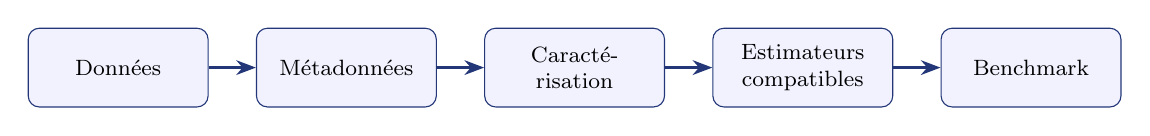
\begin{tikzpicture}[
    node distance=0.5cm and 0.6cm,
    box/.style={rectangle, rounded corners, draw=myblue, fill=blue!5,
                text width=2.05cm, align=center, minimum height=1cm, font=\footnotesize},
    arr/.style={-{Stealth[length=2.5mm]}, myblue, thick}]
\node[box] (a) {Données};
\node[box, right=of a] (b) {Métadonnées};
\node[box, right=of b] (c) {Caracté-\\risation};
\node[box, right=of c] (d) {Estimateurs compatibles};
\node[box, right=of d] (e) {Benchmark};
\draw[arr] (a)--(b);
\draw[arr] (b)--(c);
\draw[arr] (c)--(d);
\draw[arr] (d)--(e);
\end{tikzpicture}
\end{center}
\vspace{0.3cm}
\begin{tabularx}{\textwidth}{>{\RaggedRight\arraybackslash}p{0.30\textwidth} >{\RaggedRight\arraybackslash}X}
\toprule
\textbf{Bloc} & \textbf{Informations principales} \\
\midrule
Formule \& variables & Y, X, formule publiée ou reconstruite \\
Provenance & DOI dataset, DOI publication, source \\
Caractéristiques du modèle & Tâche, familles d'estimateurs compatibles \\
Structure des données & Support spatial, panel, profil $N/T$ \\
Résolution \& étendue & Unité spatiale, emprise, période \\
Reproductibilité & Code, dépôt, licence \\
\bottomrule
\end{tabularx}
\end{frame}

\begin{frame}{Une architecture pour passer à l'échelle}
\small
\textbf{La difficulté} : des centaines de sources hétérogènes (articles PDF,
packages, dépôts) à lire, croiser et vérifier : un travail manuel qui ne
tient pas à l'échelle du projet.
\vspace{0.3cm}
\begin{block}{Le principe adopté}
Maximiser les étapes \textbf{déterministes et scriptées} ; réserver l'usage
du LLM, coûteux, aux endroits où il est le plus efficace (lecture,
classement, vérification ponctuelle), jamais comme mémoire ou comme automate
de bout en bout.
\end{block}
\vspace{0.25cm}
\textbf{Ex.} :
\begin{itemize}\setlength\itemsep{0.08cm}
    \item Reconstruire la \textbf{formule} quand elle n'est pas disponible
    \item Reconstruire la \textbf{géométrie} quand elle est spécifiée sous une autre forme
    \item Le reste (DOI, $N\times T$, X\dots) : outils déterministes, gratuits, fiables
\end{itemize}
\end{frame}

\begin{frame}{Les outils de la curation (1/2) : mémoire et graphe}
\footnotesize
\begin{columns}[T]
\column{0.40\textwidth}
\textbf{LLM Wiki} : plutôt que tout relire à chaque tâche, l'assistant
construit une mémoire cumulative : des fiches de synthèse reliées entre
elles, consultables et vérifiables par un humain.
\vspace{0.2cm}

\textbf{Graphe de connaissances (KG)} : des \emph{nœuds} (article, dataset,
formule) reliés par des relations (\emph{utilise}, \emph{fournit},
\emph{documente}). Il oriente d'abord l'assistant vers les bonnes sources,
avant que le wiki ne livre une synthèse lisible.
\column{0.58\textwidth}
\centering
\resizebox{0.95\linewidth}{!}{%
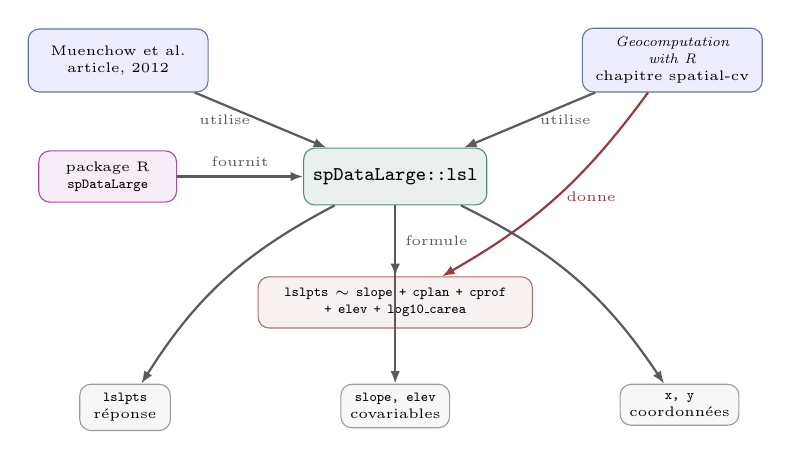
\begin{tikzpicture}[
    node distance=6mm and 8mm,
    every node/.style={font=\tiny, align=center},
    dataset/.style={draw=mygreen!80, fill=mygreen!10, rounded corners,
        minimum width=2.0cm, minimum height=0.72cm, font=\scriptsize\bfseries},
    paper/.style={draw=myblue!70, fill=blue!7, rounded corners,
        text width=2.05cm, minimum height=0.8cm},
    package/.style={draw=violet!70, fill=violet!7, rounded corners,
        minimum width=1.75cm, minimum height=0.65cm},
    formula/.style={draw=myred!75, fill=myred!7, rounded corners,
        text width=3.25cm, minimum height=0.65cm},
    varnode/.style={draw=mygray!60, fill=black!3, rounded corners,
        minimum width=1.15cm, minimum height=0.52cm},
    edge/.style={-{Latex[length=1.6mm]}, thick, mygray}
]
\node[dataset] (lsl) {\texttt{spDataLarge::lsl}};
\node[paper, above left=7mm and 12mm of lsl] (article)
    {Muenchow et al.\\article, 2012};
\node[paper, above right=7mm and 12mm of lsl] (book)
    {\emph{Geocomputation with R}\\chapitre spatial-cv};
\node[package, left=16mm of lsl] (pkg) {package R\\\texttt{spDataLarge}};
\node[formula, below=9mm of lsl] (form)
    {\texttt{lslpts} $\sim$ \texttt{slope + cplan + cprof}\\
     \texttt{+ elev + log10\_carea}};
\node[varnode, below left=7mm and 11mm of form] (y)
    {\texttt{lslpts}\\réponse};
\node[varnode, below=7mm of form] (x)
    {\texttt{slope, elev}\\covariables};
\node[varnode, below right=7mm and 11mm of form] (xy)
    {\texttt{x, y}\\coordonnées};
\draw[edge] (pkg) -- node[above]{fournit} (lsl);
\draw[edge] (article) -- node[left]{utilise} (lsl);
\draw[edge] (book) -- node[right]{utilise} (lsl);
\draw[edge,myred] (book) to[bend left=12] node[right]{donne} (form);
\draw[edge] (lsl) -- node[right]{formule} (form);
\draw[edge] (lsl) to[bend right=15] (y);
\draw[edge] (lsl) -- (x);
\draw[edge] (lsl) to[bend left=15] (xy);
\end{tikzpicture}
}
\end{columns}
\vspace{0.1cm}

{\scriptsize\textcolor{mygray}{Coupler wiki LLM et graphe de connaissances : une combinaison encore rare au moment du stage (concept publié 3 mois avant), peu faite ailleurs.}}
\end{frame}

\begin{frame}{Les outils de la curation (2/2) : lire et outiller}
\footnotesize
\textbf{GROBID} : convertit un PDF (mise en page brute) en texte structuré
(TEI) : sections, tableaux, références identifiées séparément, grâce à des
modèles entraînés sur la mise en page des articles scientifiques.
\vspace{0.2cm}

\textbf{Lecture dirigée} : une fois le TEI obtenu, chaque section est notée
selon son utilité empirique (données/modèle $>0$, théorie/simulation $<0$)
pour ne pas confondre une formule appliquée à un vrai jeu de données avec un
exemple théorique.
\vspace{0.25cm}

\textbf{Outils et compétences des agents IA} : MCP \texttt{context\_store}
pour résumer de longues sorties avant raisonnement.
\end{frame}

\begin{frame}{Rôle des LLM dans le projet}
\footnotesize
\textbf{Deux agents IA, rôles distincts} :
\begin{itemize}\setlength\itemsep{0.08cm}
    \item \textbf{Codex} : production et injection des fiches, exploration du
    dépôt, écriture des scripts R/Python du pipeline technique.
    \item \textbf{Claude} : contrôle qualité, ne modifie jamais une fiche
    lui-même.
\end{itemize}
\vspace{0.25cm}
\begin{columns}[T]
\column{0.5\textwidth}
\textbf{Un filtre scripté d'abord} : un filtre déterministe et gratuit tourne
sur \emph{tout} le corpus ; le LLM n'est appelé que sur les candidats qui ont
déjà franchi ce seuil.

\column{0.48\textwidth}
\textbf{Trois points d'intervention de Claude}
\begin{itemize}\setlength\itemsep{0.12cm}
    \item \textbf{Sélection Y/X} (bloc packages)
    \item \textbf{Vérification des candidats} (bloc entrepôts)
    \item \textbf{Contrôle qualité Tier 2} (transversal)
\end{itemize}
\end{columns}
\vspace{0.2cm}
\centering\textbf{Principe clé : l'IA propose, l'humain valide.} Aucune auto-validation.
\end{frame}

\begin{frame}{Bloc packages : vue d'ensemble}
\footnotesize
\textbf{Trois voies visées au départ} : \textit{package-first},
\textit{article-first}, \textit{dépôt-first}.
\vspace{0.2cm}

Article-first s'est révélée peu praticable. Toutefois, la recherche du
papier associé continue bien dans les deux blocs restants, chacun à sa
manière.
\vspace{0.25cm}

\textbf{Bloc 1} : entrée la plus stable, parce que les objets sont déjà
accessibles et inspectables localement (51 packages ciblés : \texttt{spdep},
\texttt{spData}, \texttt{GWmodel}, \texttt{ade4}, \texttt{geodatasets},
\texttt{libpysal}\dots).
\vspace{0.15cm}
\begin{center}
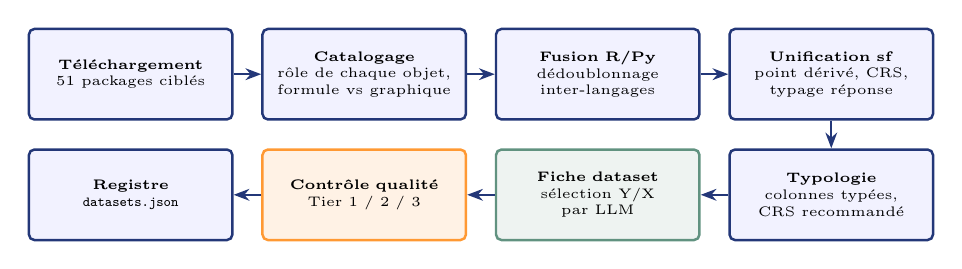
\begin{tikzpicture}[
    node distance=0.35cm and 0.35cm,
    box/.style={rectangle, rounded corners=2pt, draw=myblue, line width=0.9pt, fill=blue!5,
                text width=2.35cm, align=center, minimum height=1.15cm, font=\tiny},
    llmgen/.style={rectangle, rounded corners=2pt, draw=mygreen!75, line width=0.9pt, fill=mygreen!8,
                text width=2.35cm, align=center, minimum height=1.15cm, font=\tiny},
    llmver/.style={rectangle, rounded corners=2pt, draw=orange!80, line width=0.9pt, fill=orange!10,
                text width=2.35cm, align=center, minimum height=1.15cm, font=\tiny},
    arr/.style={-{Stealth[length=2mm]}, myblue, thick}]
\node[box] (a) {\textbf{Téléchargement}\\51 packages ciblés};
\node[box, right=of a] (b) {\textbf{Catalogage}\\rôle de chaque objet, formule vs graphique};
\node[box, right=of b] (c) {\textbf{Fusion R/Py}\\dédoublonnage inter-langages};
\node[box, right=of c] (d) {\textbf{Unification sf}\\point dérivé, CRS, typage réponse};
\node[box, below=of d] (e) {\textbf{Typologie}\\colonnes typées, CRS recommandé};
\node[llmgen, left=of e] (f) {\textbf{Fiche dataset}\\sélection Y/X par LLM};
\node[llmver, left=of f] (g) {\textbf{Contrôle qualité}\\Tier 1 / 2 / 3};
\node[box, left=of g] (h) {\textbf{Registre}\\\texttt{datasets.json}};
\draw[arr] (a)--(b); \draw[arr] (b)--(c); \draw[arr] (c)--(d);
\draw[arr] (d)--(e); \draw[arr] (e)--(f); \draw[arr] (f)--(g); \draw[arr] (g)--(h);
\end{tikzpicture}
\end{center}
\vspace{0.1cm}
{\scriptsize\textcolor{mygreen}{$\blacksquare$} LLM de génération (Y/X) \quad
{\scriptsize\textcolor{orange}{$\blacksquare$} LLM de vérification (Claude)} \quad
{\scriptsize\textcolor{myblue}{$\blacksquare$} étape scriptée}}
\end{frame}

\begin{frame}{Bloc entrepôts : deux modes de recherche \textit{dataset-first}}
\footnotesize
Dans les deux cas, on part de la \textbf{donnée}, pas du papier : le papier
associé est retrouvé \emph{après coup}, dans les métadonnées mêmes du dépôt
(\texttt{relatedIdentifiers}) : jamais l'inverse.
\vspace{0.2cm}
\begin{center}
\resizebox{\textwidth}{!}{%
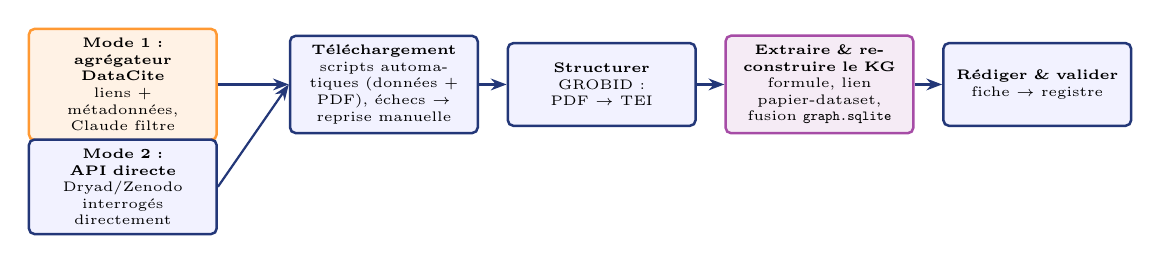
\begin{tikzpicture}[
    node distance=0.35cm and 0.35cm,
    box/.style={rectangle, rounded corners=2pt, draw=myblue, line width=0.9pt, fill=blue!5,
                text width=2.15cm, align=center, minimum height=1.05cm, font=\tiny},
    llmver/.style={rectangle, rounded corners=2pt, draw=orange!80, line width=0.9pt, fill=orange!10,
                text width=2.15cm, align=center, minimum height=1.05cm, font=\tiny},
    kgbuild/.style={rectangle, rounded corners=2pt, draw=violet!70, line width=0.9pt, fill=violet!8,
                text width=2.15cm, align=center, minimum height=1.05cm, font=\tiny},
    arr/.style={-{Stealth[length=2mm]}, myblue, thick}]
\node[llmver] (m1) at (0,0.65) {\textbf{Mode 1 : agrégateur DataCite}\\liens + métadonnées, Claude filtre};
\node[box] (m2) at (0,-0.65) {\textbf{Mode 2 : API directe}\\Dryad/Zenodo interrogés directement};
\node[box, right=0.9cm of m1] (dl) {\textbf{Téléchargement}\\scripts automatiques (données + PDF), échecs $\to$ reprise manuelle};
\node[box, right=of dl] (c) {\textbf{Structurer}\\GROBID : PDF $\to$ TEI};
\node[kgbuild, right=of c] (d) {\textbf{Extraire \& reconstruire le KG}\\formule, lien papier-dataset, fusion \texttt{graph.sqlite}};
\node[box, right=of d] (e) {\textbf{Rédiger \& valider}\\fiche $\to$ registre};
\draw[arr] (m1.east) -- (dl.west); \draw[arr] (m2.east) -- (dl.west);
\draw[arr] (dl)--(c); \draw[arr] (c)--(d); \draw[arr] (d)--(e);
\end{tikzpicture}}
\end{center}
\vspace{0.1cm}
{\scriptsize\textcolor{orange}{$\blacksquare$} LLM de vérification (Claude) \quad
\textcolor{violet}{$\blacksquare$} reconstruction du KG (\texttt{run\_all.py}) \quad
\textcolor{myblue}{$\blacksquare$} étape scriptée}

\vspace{0.15cm}
{\scriptsize\textcolor{mygray}{Une voie symétrique « journal-first » (partir d'une revue, chercher le dataset ensuite) existe en complément, gardée pour les domaines où elle reste rentable.}}
\end{frame}

% ============================================================
\section{Estimateurs et évaluation}
% ============================================================
\begin{frame}{Pourquoi ces familles d'estimateurs}
\small
Les données spatiales posent deux problèmes distincts, à diagnostiquer
ensemble sans les confondre (Cliff \& Ord, 1973 ; synthèse en français :
Le Gallo, 2002, 2004) :
\begin{itemize}
    \item \textbf{Dépendance spatiale} : les observations proches ne sont pas indépendantes.
    \item \textbf{Hétérogénéité spatiale} : la relation entre $Y$ et $X$ peut varier selon le lieu.
\end{itemize}
\vspace{0.3cm}
\begin{block}{Un piège de diagnostic}
Un indice de Moran significatif sur les résidus ne signifie pas toujours
qu'il faut introduire une dépendance spatiale explicite : il peut aussi
signaler une \textbf{mauvaise spécification} (non-linéarité omise,
interaction non représentée).
\end{block}
\end{frame}

\begin{frame}{Estimateurs (1/4) : Références globales et prédictives}
\footnotesize
\textbf{Régression linéaire ordinaire (OLS)}, référence la plus simple :
\[
\mathbf{y}=X\boldsymbol{\beta}+\boldsymbol{\varepsilon}
\]

\textbf{GAM}, généralisation terme à terme d'OLS :
\[
y_i=\beta_0+\sum_{k=1}^{p} f_k(x_{ik})+\varepsilon_i
\]
$f_k$ linéaire redonne OLS.

\textbf{GAM spatial}, cas intermédiaire avec un lisseur spatial continu :
\[
y_i=\beta_0+\sum_{k=1}^{p}\beta_kx_{ik}+s(u_i,v_i)+\varepsilon_i
\]
Les coefficients $\beta_k$ restent communs à tout le territoire ; seul le
terme $s(u,v)$ capture un effet spatial continu.
\vspace{0.15cm}

MARS, Random Forest et XGBoost suivent la même logique, sans intégrer la
dimension spatiale.
\end{frame}

\begin{frame}{Estimateurs (2/4) : Dépendance spatiale}
\small
Exploitent une matrice de poids spatiaux $W$ (contiguïté, distance,
$k$-plus-proches-voisins).
\vspace{0.2cm}

\textbf{SAR (spatial autoregressive lag)}, ex. mimétisme :
\[
\mathbf{y}=\rho W\mathbf{y}+X\boldsymbol{\beta}+\boldsymbol{\varepsilon}
\]
\vspace{0.1cm}

\textbf{SEM (spatial error model)} : dépendance spatiale dans le terme d'erreur.
\[
\mathbf{y}=X\boldsymbol{\beta}+\mathbf{u},\qquad \mathbf{u}=\lambda W\mathbf{u}+\boldsymbol{\varepsilon}
\]
\vspace{0.1cm}

\textbf{SDM (spatial Durbin model)} : effets de débordement.
\[
\mathbf{y}=\rho W\mathbf{y}+X\boldsymbol{\beta}+WX\boldsymbol{\theta}+\boldsymbol{\varepsilon}
\]
\vspace{0.1cm}

\textbf{spboost} : boosting fonctionnel sur une structure SAR, SEM ou
SARAR : relation flexible entre réponse et covariables, sélection
automatique de variables.
\end{frame}

\begin{frame}{Estimateurs (3/4) : Hétérogénéité spatiale et modèles locaux}
\small
Au lieu d'un coefficient unique, la relation entre $Y$ et $X$ peut varier
selon le lieu.
\vspace{0.2cm}

\textbf{GWR (geographically weighted regression)} :
\[
y_i=\hat{\beta}_0(u_i,v_i;w_{ij})+\sum_{k=1}^{p}\hat{\beta}_k(u_i,v_i;w_{ij})x_{ik}+\varepsilon_i,
\qquad w_{ij}=K\!\left(\tfrac{d_{ij}}{h}\right)
\]
\vspace{0.2cm}

\textbf{MGWR} prolonge ce principe : un voisinage (bande passante, $h_k$)
différent par covariable.
\vspace{0.2cm}

\textbf{GWR + SAR (MGWRSAR)} articule dépendance autorégressive \emph{et}
coefficients localement variables, au croisement des deux familles
précédentes.
\end{frame}

\begin{frame}{Estimateurs (4/4) : Filtres spectraux}
\small
\textbf{Filtrage spectral (ESF / RESF)} : extrait des vecteurs propres de
Moran plutôt qu'un unique paramètre autorégressif :
\[
\mathbf{y}=X\boldsymbol{\beta}+E\boldsymbol{\gamma}+\boldsymbol{\varepsilon}
\]
\vspace{0.2cm}

{\scriptsize\textcolor{mygray}{28 estimateurs/variantes recensés au total, répartis sur 6 familles.}}
\end{frame}

\begin{frame}{Le package \texttt{spatialtidymodels}}
\small
Pour comparer les estimateurs entre eux, on a développé un package
d'intégration étendant \texttt{tidymodels} aux estimateurs spatiaux
proposé, appelé \texttt{spatialtidymodels}.
\vspace{0.2cm}

L'enjeu est de faciliter le passage des objets spatiaux nécessaires aux
estimateurs et la gestion de schémas de cross-validation adaptés.
\vspace{0.25cm}

\textbf{Objets spatiaux nécessaires aux estimateurs} :
\begin{itemize}
    \item Géométrie
    \item Matrice d'interaction spatiale $W$
    \item Noyaux de lissage spatial et bande passante
    \item Matrice de vecteurs propres pour le filtrage spectral
\end{itemize}
\end{frame}

% ============================================================
\begin{frame}{Schémas de cross-validation}
\small
\begin{tabularx}{\textwidth}{>{\bfseries\RaggedRight\arraybackslash}p{0.24\textwidth} X}
\toprule
Schéma & Principe \\
\midrule
\texttt{holdout\_10pct} & Séparation aléatoire simple : 90\,\% apprentissage, 10\,\% test. \\
\addlinespace
\texttt{near\_prediction} & Un point test par cellule quadtree et par répétition, sans remise. Approxime un LOOCV spatial à moindre coût. \\
\addlinespace
\texttt{block\_spatial} & Blocs spatiaux répartis en plis ; le plus exigeant. \\
\bottomrule
\end{tabularx}
\vspace{0.3cm}
Trois schémas supplémentaires existent dans le package, moins centraux au
benchmark actuel :
\begin{itemize}
    \item \texttt{vfold\_cv} : validation croisée standard par $k$ folds, aveugle à l'espace.
    \item \texttt{in\_sample} : pas de test séparé, diagnostic rapide, pas une évaluation.
    \item \texttt{custom} : l'utilisateur fournit son propre découpage \texttt{rsample}.
\end{itemize}
\end{frame}

% ============================================================
\section{Résultats}
% ============================================================
\begin{frame}{État de la banque : vue d'ensemble}
\footnotesize
\centering
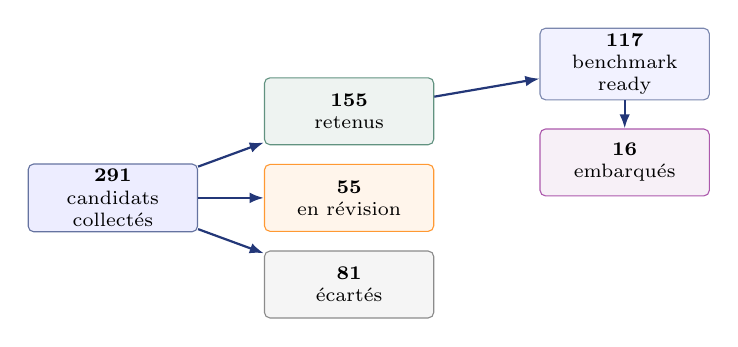
\begin{tikzpicture}[
    metric/.style={rounded corners=2pt, minimum width=2.15cm,
        minimum height=0.85cm, text width=1.95cm, align=center,
        font=\scriptsize, inner sep=2pt},
    flow/.style={-{Latex[length=1.8mm]}, thick, myblue}
]
\node[metric, draw=myblue!70, fill=blue!7] (all) at (0,0)
    {\textbf{291}\\candidats\\collectés};
\node[metric, draw=mygreen!75, fill=mygreen!8] (yes) at (3.0,1.1)
    {\textbf{155}\\retenus};
\node[metric, draw=orange!80, fill=orange!8] (rev) at (3.0,0)
    {\textbf{55}\\en révision};
\node[metric, draw=mygray!70, fill=black!4] (no) at (3.0,-1.1)
    {\textbf{81}\\écartés};
\node[metric, draw=myblue!60, fill=blue!5] (ready) at (6.5,1.7)
    {\textbf{117}\\benchmark\\ready};
\node[metric, draw=violet!65, fill=violet!6] (embarq) at (6.5,0.45)
    {\textbf{16}\\embarqués};
\draw[flow] (all) -- (yes); \draw[flow] (all) -- (rev); \draw[flow] (all) -- (no);
\draw[flow] (yes) -- (ready); \draw[flow] (ready) -- (embarq);
\end{tikzpicture}

\vspace{0.15cm}
\begin{block}{\footnotesize « Embarqué », qu'est-ce que ça veut dire ?}
\footnotesize
Le jeu est directement inclus et prêt à l'usage dans le package, sans
téléchargement. Les autres jeux déjà constitués (150+) restent accessibles
via une commande qui les télécharge depuis un dépôt public externe, mais ne
sont pas embarqués directement.
\end{block}
\vspace{0.1cm}
{\scriptsize\textcolor{mygray}{Raison : embarquer tous les jeux alourdirait trop le poids du package sur le CRAN.}}
\end{frame}

\begin{frame}{Premier benchmark réel : dispositif}
\small
\textbf{9 jeux} de moins de 2\,000 observations (sur les 16 déjà embarqués),
\textbf{10 estimateurs}, \textbf{2 schémas} d'évaluation.
\vspace{0.2cm}
\texttt{ols}, \texttt{gam\_spatial}, \texttt{sar}, \texttt{sem}, \texttt{sdm},
\texttt{GWR}, \texttt{spboost\_bspa\_sar\_ml}, \texttt{spboost\_bspa\_sem\_ml},
\texttt{random\_forest}, \texttt{xgboost}
\vspace{0.2cm}

Comparaison par amélioration relative de RMSE :
\[
\Delta RMSE_i = 100\times\frac{RMSE_{\mathrm{ref},i}-RMSE_{\mathrm{var},i}}{RMSE_{\mathrm{ref},i}}
\]
\vspace{0.1cm}
{\scriptsize\textcolor{mygray}{Pour l'instant, OLS sert de référence ; à terme, ce sera le meilleur estimateur du moment, pour que tout nouvel estimateur se compare au meilleur, pas à OLS.}}
\vspace{0.15cm}

Verdict fondé sur 4 critères cumulatifs (taux de victoires, test de Wilcoxon,
médiane positive, dégradations limitées) : pas une simple moyenne de RMSE.
\end{frame}

\begin{frame}{Résultats : \texttt{near\_prediction}}
\scriptsize
\begin{tabularx}{\textwidth}{>{\RaggedRight\arraybackslash}p{0.24\textwidth} X r r}
\toprule
Famille & Estimateur & RMSE méd. relative & Durée méd. (s) \\
\midrule
MGWRSAR & \texttt{mgwrsar\_gwr} & $\star$\,\textbf{0,85} & 0,55 \\
Machine learning & \texttt{gam\_spatial} & 0,89 & 0,57 \\
Boosting & \texttt{spboost\_bspa\_sar\_ml} & 0,91 & 4,07 \\
Machine learning & \texttt{random\_forest} & 0,95 & $\star$\,\textbf{0,30} \\
Boosting & \texttt{spboost\_bspa\_sem\_ml} & 0,97 & 4,79 \\
Machine learning & \texttt{xgboost} & 0,98 & 0,67 \\
Baseline & \textbf{\texttt{ols} (référence)} & \textbf{1,00} & 0,45 \\
Spatial econometrics & \texttt{sem\_error} & 1,06 & 4,99 \\
Spatial econometrics & \texttt{sdm\_mixed} & 1,10 & 4,62 \\
Spatial econometrics & \texttt{sar\_lag} & 1,23 & 5,08 \\
\bottomrule
\end{tabularx}
\vspace{0.2cm}
{\scriptsize $\star$ meilleure valeur par critère.}
\vspace{0.1cm}

\textbf{Trois familles} réduisent la RMSE de 3 à 15\,\% : boosting spatial, GWR,
\texttt{gam\_spatial}. \textbf{SAR/SDM} perdent et coûtent
4 à 5\,s par ajustement contre moins d'1\,s pour la référence.
\end{frame}

\begin{frame}{Pourquoi SAR/SEM/SDM échouent-ils autant ?}
\small
\textbf{Origine du modèle dans la publication} :
\vspace{0.2cm}

\begin{tabularx}{\textwidth}{>{\RaggedRight\arraybackslash}p{0.4\textwidth} X}
\toprule
Origine & Jeux du benchmark \\
\midrule
GWR (hétérogénéité) & georgia, ewhp, london\_hp, dub\_voter \\
Dépendance (SAR/SEM) & wang\_henan, lasrosas \\
Aucun modèle spatial & boston\_housing, seshat \\
\bottomrule
\end{tabularx}
\vspace{0.3cm}

6 des 8 jeux ne sont pas d'origine ``dépendance spatiale'' :
SAR/SEM/SDM y sont testés hors du contexte pour lequel ils ont été conçus.
\end{frame}

\begin{frame}{Le tableau de bord interactif}
\begin{columns}[T]
\column{0.52\textwidth}
\centering
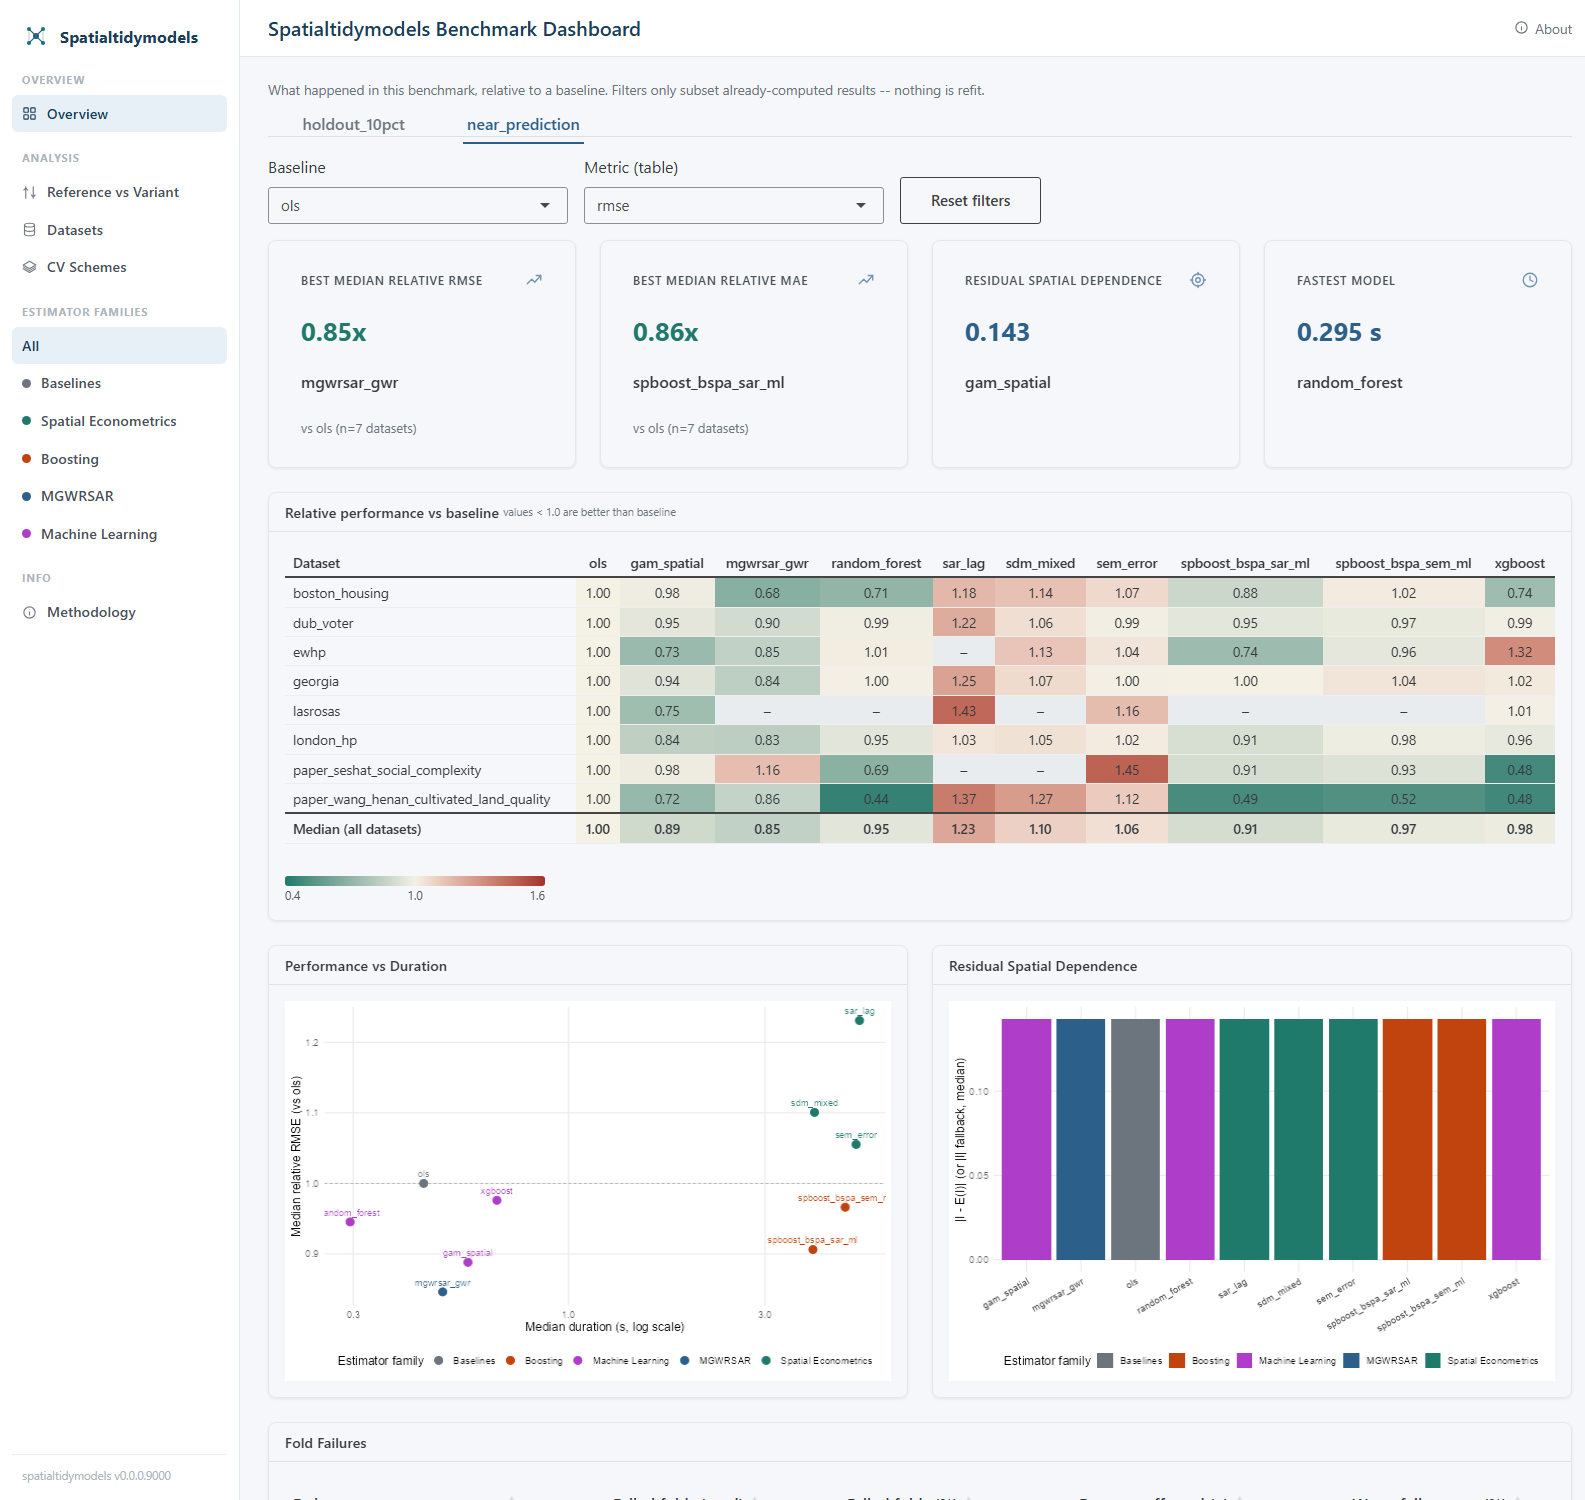
\includegraphics[width=\linewidth,height=6.2cm,keepaspectratio]{dashboard_overview_near.png}
\column{0.45\textwidth}
\footnotesize
Page \emph{Overview}, schéma \texttt{near\_prediction}, 5 pages : vue
d'ensemble, référence vs variante, détail par jeu, par schéma, méthodologie.
\vspace{0.3cm}

\begin{block}{\footnotesize Au-delà de la médiane}
\scriptsize Le tableau de bord permet d'explorer la performance \textbf{jeu par jeu}
au-delà de la médiane agrégée, pour comprendre dans quelles conditions
(taille, densité spatiale...) un estimateur donné est le plus performant.
C'est cette diversité de jeux qui rend cette lecture possible.
\end{block}
\end{columns}
\end{frame}

% ============================================================
\section{Conclusion}
% ============================================================
\begin{frame}{Conclusion et perspectives}
\footnotesize
\textbf{Ce qui a été construit} : une chaîne complète, de la collecte à la
restitution des résultats, mise à l'épreuve sur un premier benchmark réel qui
fonctionne de bout en bout.
\vspace{0.06cm}

\textbf{Suite immédiate}
\begin{itemize}
    \item Relancer les pipelines de collecte pour élargir la banque.
    \item Étendre le benchmark au schéma \texttt{block\_spatial} et aux jeux
    volumineux écartés du premier lot, via un sous-échantillonnage par
    territoire et par période plutôt qu'un traitement en un seul bloc.
\end{itemize}
\vspace{0.04cm}
\textbf{À terme}
\begin{itemize}
    \item Le package reste léger ; la banque complète sera déposée séparément (entrepôt ouvert, versionné).
    \item Un \emph{data paper} (\textit{Data Descriptor}, \textit{Scientific Data}), incluant une étude bibliométrique Monte-Carlo vs données réelles ; citée dans la durée, contrairement à un article de méthode.
    \item Extensions futures : réponses binaires, comptages, panels, probit spatiaux.
\end{itemize}
\end{frame}

\section*{}
\begin{frame}[plain]
  \begin{center}
    {\Huge Merci de votre attention}\\[1em]
    {\large Johnny D'OLIVEIRA}\\[0.3em]
    Aix-Marseille School of Economics\\[0.3em]
    INRAE, Unité Écodéveloppement
  \end{center}
\end{frame}

\end{document}
